\section{Results}
\label{sec:results}

The results follow the research questions: the two-level account (Section~\ref{subsec:res_levels}, RQ1), the scalar feedback gate (Section~\ref{subsec:res_scalar}, RQ2), the directional feedforward gate (Section~\ref{subsec:res_directional}, RQ3), a synthesis of the two momentum crosses (Section~\ref{subsec:res_regimeflip}), and the CIFAR-10 generalisation of both gates (Section~\ref{subsec:res_cifar}, RQ4).

\paragraph{Reading the tables.}
Depth is in percentage points (pp): a depth of $19.5$ means the worst past-task evaluation falls $19.5$ points below its pre-switch baseline. The end-referenced area \texttt{gap\_area\_end} integrates the excursion below the level each task settles at; its conventions, and the caveat that cross-condition areas must be read together with final accuracy, are stated once in Section~\ref{subsec:metrics}. Values are mean $\pm$ standard deviation over five seeds (three for the CIFAR generalisation block); comparisons follow the Wilcoxon convention of Section~\ref{subsec:metrics}, quoting a $p$-value only where seeds disagree. The full metric set for every condition is in Appendix~\ref{app:full_results}.

\subsection{The Two Levels, Separated (RQ1)}
\label{subsec:res_levels}

RQ1 asks whether the transient separates into a deterministic arc of the intended trajectory and overshoot of whatever path is actually followed. The ladder of Section~\ref{subsec:ladder} answers it as a limit rather than as a comparison: with the objective, the update rule, $\theta_0^*$ and the replay buffer bit-identical across rungs and only $\eta$ varying at matched flow time, the four rungs are four discretisations of one and the same intended trajectory, and whatever survives $\eta \rightarrow 0$ is that trajectory. Depth is $\eta$-invariant and quoted in pp throughout; the area is the flow-time integral $A_\tau = \eta A_{\text{steps}}$, the only form comparable across rungs (Section~\ref{subsec:metrics}).

\begin{figure*}[t]
    \centering
    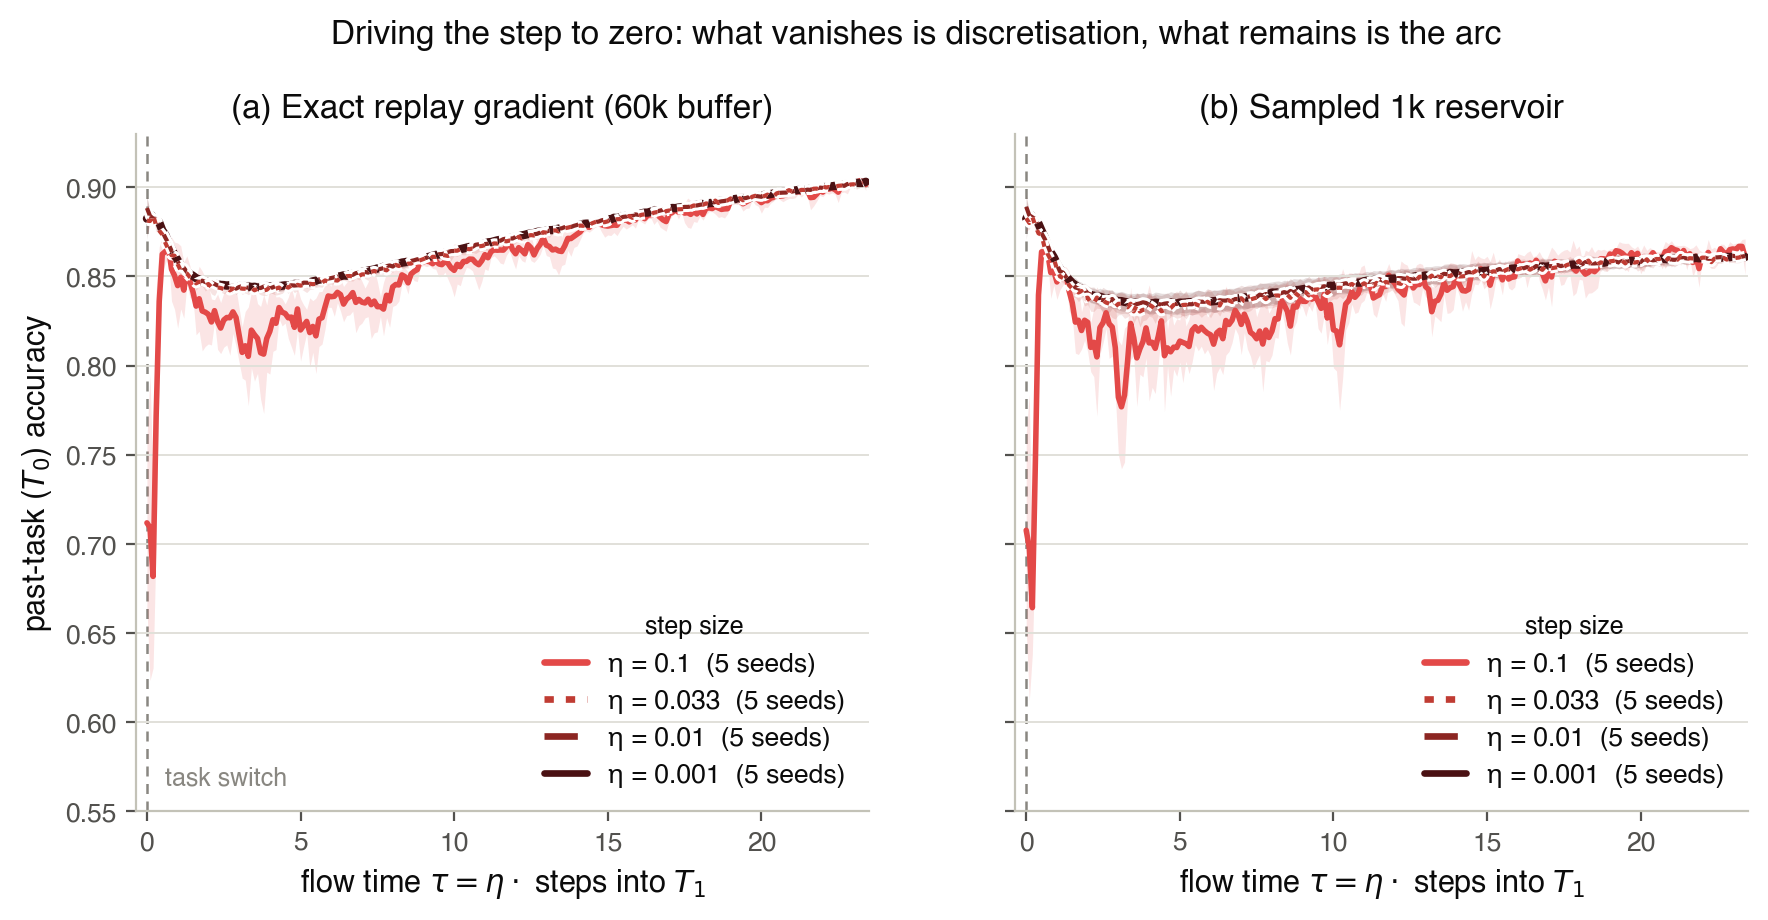
\includegraphics[width=0.86\linewidth]{img/results/ladder/step_size_ladder.png}
    \caption{The step-size ladder at momentum $0$: past-task ($T_0$) accuracy against flow time $\tau = \sum_t \eta$, seed mean with $\pm$std bands, $\tau{=}0$ the task switch. Every rung covers the same $\tau = 23.5$ from the same frozen $\theta_0^*$ and the same buffer, so within a panel $\eta$ is the only difference. (a) exact $60$k replay gradient, (b) the $1$k reservoir of the standard protocol. What the reader should see is a limit that is reached and is not zero. The standard operating point (light, $\eta = 0.1$) leaves the other three within its first two steps, drops ${\approx}20$ pp, and spends the rest of the task jittering back; the three finer rungs (dark: $\eta = 0.1/3$ and $\eta = 0.01$ dashed, $\eta = 0.001$ solid) have no boundary spike at all, and overlap so closely that linestyle rather than colour is what separates them. What they do have is a smooth dip-and-recover bend that neither the smaller step nor the exact gradient removes: the arc.}
    \label{fig:ladder}
\end{figure*}

\paragraph{The ladder converges, and not on zero.}
At momentum $0$ the three finest rungs are all but the same run. On the exact arm depth falls $22.3 \rightarrow 4.2 \rightarrow 3.9 \rightarrow 3.8$ pp for $\eta = 0.1 \rightarrow 0.1/3 \rightarrow 0.01 \rightarrow 0.001$, with the flow-time area at $0.590 \rightarrow 0.360 \rightarrow 0.346 \rightarrow 0.341$ and ACC at $0.895 \rightarrow 0.897 \rightarrow 0.897 \rightarrow 0.898$; on the sampled arm, $22.9 \rightarrow 5.6 \rightarrow 4.9 \rightarrow 4.7$ pp, area $0.577 \rightarrow 0.293 \rightarrow 0.275 \rightarrow 0.270$, ACC $0.874 \rightarrow 0.876 \rightarrow 0.877 \rightarrow 0.877$ (all sixteen cells with their full metric set in Appendix~\ref{app:ladder_full}).
The last step down each ladder, a further tenfold cut from $\eta = 0.01$ to $\eta = 0.001$, moves depth by $0.1$ and $0.2$ pp against the $18.1$ and $17.3$ pp the first step removes, and the trajectories themselves coincide: the largest separation between the $\eta = 0.1/3$ and $\eta = 0.01$ curves anywhere on the common flow-time grid is $0.007$ (exact) and $0.006$ (sampled) in accuracy, against $0.201$ and $0.219$ for $\eta = 0.1$, both attained at $\tau \approx 0.2$, inside the coarse rung's first two steps (Figure~\ref{fig:ladder}). These residual differences are small but not noise: three of the four contrasts between those two rungs are unanimous in sign across seeds ($p = 0.0625$; the exception is the sampled area, four of five, $p = 0.125$), which is what an $O(\eta)$ remainder should look like. Extrapolating $A(\eta) = A_0 + k\eta$ through the fine rungs alone puts the limit at $3.8$ pp of depth and $0.34$ of area on the exact arm, $4.7$ pp and $0.27$ on the sampled one. That positive limit is RQ1's answer: an excursion that survives both the exact gradient and the vanishing step has no Level-Two driver left to attribute it to, and it is the arc of Section~\ref{subsec:trajectory_problem} measured rather than inferred. The all-rung least-squares fit is not the estimate to read here: over a $100\times$ lever arm the line is pinned by the coarse rung, whose excess inflates the slope to $k \approx 2.0$, pulls the depth intercept down to $1.5 \pm 1.1$ pp, and leaves a largest residual of $3.8$ pp, the size of the very quantity being estimated. That is the linear model reporting that one of its four points does not belong to its regime.

\paragraph{The coarse rung sits above the line.}
How far it sits above is the sharpest single number the block produces: $17.2$ pp of depth and $0.19$ of area on the exact arm, $15.6$ pp and $0.24$ on the sampled one. This excess is by construction what the $O(\eta)$ model cannot account for, and it is the discrete instability itself, so between two thirds and three quarters of the depth measured at the standard operating point is not a property of the trajectory the optimiser is following. It is not estimator noise either: the departure on the exact arm, where the replay gradient carries no sampling error at all, is the larger of the two in depth. This is also where the ladder settles what the boundary imbalance is. The imbalance is identical at every rung, the same near-zero replay gradient meeting the same large new-task gradient at the same $\theta_0^*$, since a rescaling of $\eta$ leaves the vector field untouched; yet the spike it produces is gone by $\eta = 0.1/3$ and the excursion that remains is smooth. The imbalance is Level-One terrain, and the acute driver of the drop is the step size that meets it, exactly the division of labour Section~\ref{subsec:trajectory_problem} assigns them. The measured limit does qualify the metric mapping of that section, however: depth is overshoot-dominated at the operating point, but it is not overshoot alone, because the arc still registers $3.8$ pp of depth once the overshoot is gone.

\paragraph{Accuracy is not what the limit costs.}
Nothing on the ladder is traded away for the smaller gap. ACC is flat to slightly rising down both arms ($0.895 \rightarrow 0.898$ exact, $0.874 \rightarrow 0.877$ sampled), and min-ACC, the worst single evaluation of the run, improves sharply, $0.658 \rightarrow 0.843$ and $0.653 \rightarrow 0.834$. ($\mathrm{WP}_{100}$ falls, $0.453 \rightarrow 0.376$ and $0.454 \rightarrow 0.369$, but it is a fixed hundred-\emph{step} horizon and therefore spans a hundredth of the flow time at $\eta = 0.001$; the decline is a units artefact of the reparametrisation and is not read as a plasticity cost.) What the limit costs is compute. Matched flow time makes the epoch count scale as $1/\eta$, so the $\eta = 0.001$ rung removes $18.5$ pp of depth at a hundred times the training of the operating point, and it removes only the overshoot. This is the bar the gates of RQ2 and RQ3 have to clear: not lowering the gap, which the step size already does with no method at all, but lowering it at the standard step size and in the standard number of steps.

\paragraph{Under momentum the ladder converges too, on an arc of its own.}
Momentum multiplies the asymptotic step by $1/(1-\mu)$, so the four rungs sit at effective steps $1.0$, $0.33$, $0.1$ and $0.01$, and only the last of these reaches the range in which the $\mu = 0$ leg had settled. It does reach it. Depth falls $14.1 \rightarrow 9.9 \rightarrow 5.0 \rightarrow 2.7$ pp on the exact arm (area $0.301 \rightarrow 0.122 \rightarrow 0.061 \rightarrow 0.040$, ACC $0.965 \rightarrow 0.973$, min-ACC $0.814 \rightarrow 0.928$) and $15.4 \rightarrow 10.1 \rightarrow 5.4 \rightarrow 4.6$ pp on the sampled one (area $0.105 \rightarrow 0.021 \rightarrow 0.0034 \rightarrow 0.0006$, ACC $0.929 \rightarrow 0.942$, min-ACC $0.802 \rightarrow 0.910$). The fine-rung extrapolation puts the limit at $2.6$ pp of depth on the exact arm and $4.1$ pp on the sampled one, only $0.1$ and $0.5$ pp below the finest rung actually run, so this leg has an arc and the bottom of the ladder is close to it. What remains true of the earlier reading is narrower than it was: the coarse rung's departure is still \emph{negative} ($-10.3$ pp exact, $-6.2$ pp sampled), lying below the line through the fine rungs rather than above it as at $\mu = 0$, so the all-rung fit is still not the estimate to read. The $O(\eta)$ model breaks down at the coarse end of both legs; under momentum it breaks down by saturating rather than by exploding.

\paragraph{Momentum is not simply a longer step.}
The grid now provides two matched-effective-step diagonals, and together they say what one alone could not. At effective step $0.1$, $(\eta = 0.01, \mu = 0.9)$ against $(\eta = 0.1, \mu = 0)$ separates widely, $5.0$ pp / $0.061$ / $0.972$ against $22.3$ pp / $0.590$ / $0.895$ on the exact arm; at effective step $0.01$, $(\eta = 0.001, \mu = 0.9)$ against $(\eta = 0.01, \mu = 0)$ reads $2.7$ pp / $0.040$ / $0.973$ against $3.9$ pp / $0.346$ / $0.897$. The depth separation collapses from $17.3$ to $1.2$ pp as the matched step shrinks, which is what two legs approaching their own $\eta \rightarrow 0$ limits must do; the area separation does not, staying eightfold at the finest matched pair. What differs between the legs is therefore the shape of the residual excursion and not only its scale. This remains the secondary read Section~\ref{subsec:ladder} calls it: the legs warm-start from anchors trained at their own momentum and settle some seven accuracy points apart, so comparing their levels compares two operating points.

\paragraph{Momentum's arc is depth without tail.}
The within-leg contrast is both the safer comparison and the sharper one. On the sampled arm the momentum leg's flow-time area falls by more than two orders of magnitude across the ladder, $0.105 \rightarrow 0.0006$, and extrapolates to zero ($-0.001$), while its depth converges on $4.1$ pp. In the limit the transient that survives under momentum is a dip that recovers almost at once: it keeps the instantaneous drop and loses the hanging tail. The $\mu = 0$ arc keeps both, $4.7$ pp of depth and $0.27$ of area that no further shortening of the step removes. Of the two-part measure of Section~\ref{subsec:metrics}, then, momentum leaves essentially only the depth term standing.

\paragraph{The coarse rung reproduces the operating point in distribution.}
$\eta = 0.1$ on the sampled arm is the standard operating point, but it is not the archived vanilla-ER reference run (D1, Appendix~\ref{app:curr_full}) and is not paired with it: the ladder skips $T_0$ training so that every cell can share one $\theta_0^*$, which leaves the two protocols on different RNG streams and hence with different buffer contents seed for seed. Their distributions agree, $22.9 \pm 4.2$ against $19.5 \pm 4.1$ pp of depth and $5.77 \pm 0.80$ against $6.27 \pm 0.47$ of step-axis area, one-standard-deviation intervals overlapping on both. That is a check that warm-starting has not moved the operating point, and nothing stronger than that.

\paragraph{What the gates inherit.}
RQ1 therefore hands on a measured quantity rather than a hypothesis. At momentum $0$ the arc is $3.8$ pp of depth and $0.34$ of flow-time area at ACC $0.898$ on the exact arm ($4.7$ pp / $0.27$ / $0.877$ sampled): a residual excursion that neither the exact gradient nor any further shortening of the step reaches, because it is not a discretisation error but the path the optimiser was following all along. Removing it requires changing the path, which is what the two gates attempt, and at the standard step size, where the ladder's own remedy is not available.

\subsection{The Scalar Feedback Gate (RQ2)}
\label{subsec:res_scalar}

Table~\ref{tab:res_curriculum} reports the curriculum sweep at both momentum settings against vanilla ER. The momentum-off leg tests the schedule in isolation; the momentum-on leg is the practically relevant regime.

\begin{table*}[htbp]
    \centering
    \small
    \resizebox{\textwidth}{!}{%
        \begin{tabular}{l ccc ccc}
            \hline
                                                 & \multicolumn{3}{c}{Momentum $0.0$} & \multicolumn{3}{c}{Momentum $0.9$}                                                                                              \\
            Condition                            & \texttt{gap\_depth} (pp)           & \texttt{gap\_area\_end}            & ACC               & \texttt{gap\_depth} (pp) & \texttt{gap\_area\_end} & ACC               \\
            \hline
            Vanilla ER (baseline)                & $19.5 \pm 4.1$                     & $6.3 \pm 0.5$                      & $0.873 \pm 0.005$ & $15.9 \pm 2.6$           & $1.0 \pm 0.2$           & $0.928 \pm 0.003$ \\
            C3: Linear $N{=}200$                 & $14.3 \pm 4.6$                     & $1.8 \pm 0.6$                      & $0.828 \pm 0.025$ & $6.2 \pm 0.6$            & $0.1 \pm 0.0$           & $0.925 \pm 0.007$ \\
            C4: Adaptive                         & $12.8 \pm 2.9$                     & $2.2 \pm 0.5$                      & $0.833 \pm 0.025$ & $2.5 \pm 0.5$            & $0.3 \pm 0.1$           & $0.917 \pm 0.001$ \\
            C7: Adaptive $\lambda_{\min}{=}0.20$ & $13.9 \pm 3.4$                     & $2.7 \pm 0.6$                      & $0.837 \pm 0.031$ & $3.7 \pm 0.4$            & $0.0 \pm 0.0$           & $0.931 \pm 0.002$ \\
            \hline
        \end{tabular}%
    }
    \caption{$\lambda$-curriculum key conditions on rot-MNIST against vanilla ER, at momentum $0.0$ and $0.9$; five seeds: the longest linear ramp (C3), the pure adaptive schedule (C4), and the practical configuration (C7). The scalar feedback gate reaches a few points of depth at matched accuracy only in the momentum-on regime it is intended for. The full sweep (C1--C7), with vanilla ER's full metric row as the reference, is in Appendix~\ref{app:curr_full}.}
    \label{tab:res_curriculum}
\end{table*}

\paragraph{The schedule works as predicted, at a momentum-$0$ price.}
At momentum $0$, mean gap depth falls monotonically with the ramp length, $17.5 \rightarrow 16.2 \rightarrow 14.3$ pp at $N = 50, 100, 200$, as the $O(1/N)$ bound of Equation~\eqref{eq:bound} predicts, though successive lengths lie within the seed spread and the reduction is bought with accuracy ($0.851 \rightarrow 0.844 \rightarrow 0.828$) and a stretched tail (per-condition metrics in Appendix~\ref{app:curr_full}). The depth that remains, still in the mid-teens, is the untouched chronic driver: the schedule times the push but leaves the finite-buffer replay estimate exactly as noisy as vanilla's, so the worst evaluation keeps arriving as a late noise-driven drop, a floor no ramp length can pass and only the exact-gradient diagnostic removes (C8, Table~\ref{tab:res_c8}). The two remaining ingredients behave as designed but earn their keep only under momentum. At momentum $0$ the adaptive signal removes the knob $N$ and changes nothing else, $12.8$ pp / $2.2$ / $0.833$ against the longest linear ramp's $14.3$ pp / $1.8$ / $0.828$, with seeds split on the depth difference ($p = 0.44$); that null is specific to this momentum setting, and the momentum leg below separates the same pair unanimously in the adaptive schedule's favour. The $\lambda_{\min}$ floor is likewise inert here, $13.9$ pp / $2.7$ / $0.837$ at $\lambda_{\min}{=}0.20$ against $12.8$ pp / $2.2$ / $0.833$ without it, because early $T_1$ progress at momentum $0$ is set by the large boundary gradient the small floor cannot redirect. The momentum-$0$ curves of Figure~\ref{fig:c_curves} (dashed) show the underlying trade: a shallower past-task dip than vanilla (a), paid for in slower early $T_1$ learning (b).

\begin{figure*}[t]
    \centering
    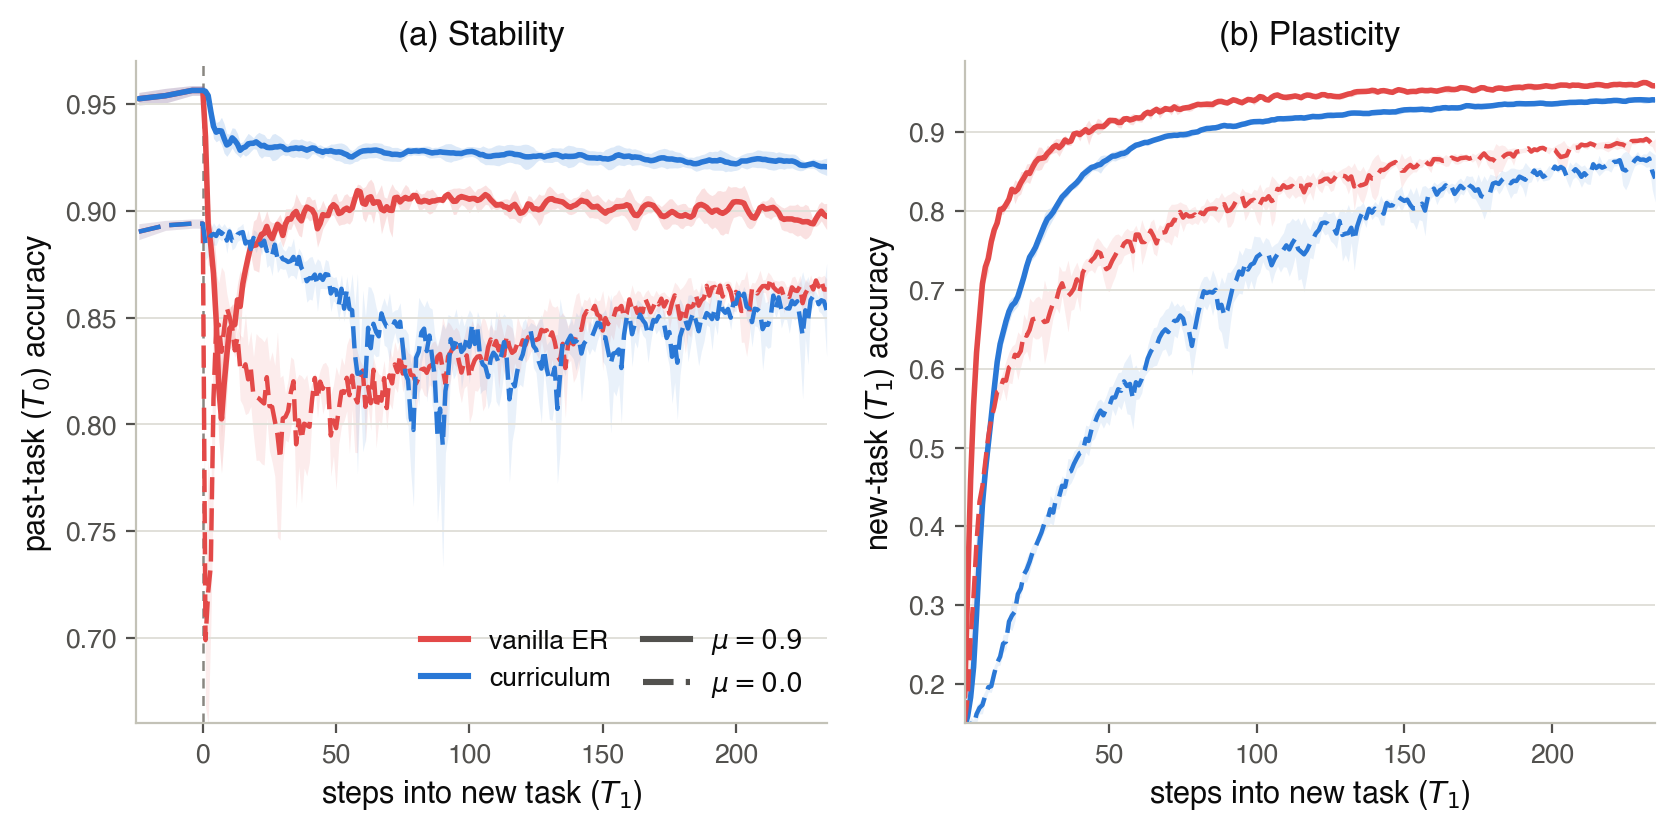
\includegraphics[width=0.85\linewidth]{img/results/curriculum/curriculum.png}
    \caption{The scalar feedback gate and momentum's two roles: per-step accuracy across the rot-MNIST switch, seed mean with $\pm$std bands, for vanilla ER (red) and the practical adaptive curriculum $\lambda_{\min}{=}0.20$ (blue), each at momentum $0.9$ (solid) and $0.0$ (dashed). \textbf{(a) Stability ($T_0$):} only curriculum-with-momentum (solid blue) holds the past task near its plateau through the switch; momentum barely dents vanilla's spike, and both methods open a deep, jittery gap without it (dashed). \textbf{(b) Plasticity ($T_1$):} at momentum $0$ the curriculum slows early new-task learning (dashed blue), the plasticity debt that momentum pays back (solid blue).}
    \label{fig:c_curves}
\end{figure*}

\paragraph{The bar is the ladder's, and at momentum $0$ the gate does not clear it.}
Lowering the gap is not by itself the gate's claim, because the step size lowers it with no method at all; the claim has to be that the gate lowers it at the standard step size and in the standard number of steps (Section~\ref{subsec:res_levels}). Nor is there an accuracy handicap to discount from the ladder's numbers: ACC is flat to rising down both arms and min-ACC improves sharply, so what the ladder charges is compute, the epoch count scaling as $1/\eta$ at matched flow time. Read against that bar on the matched $1$k arm at momentum $0$, the curriculum loses on everything but the budget. C7 leaves $13.9$ pp of depth at ACC $0.837$ and min-ACC $0.743$ in one epoch at $\eta = 0.1$; the $\eta = 0.01$ rung leaves $4.9$ pp at ACC $0.877$ and min-ACC $0.832$ in ten. Measured against its own protocol's reference the schedule removes $5.6$ pp of vanilla ER's $19.5$ and spends $3.6$ pp of ACC doing it ($0.873 \rightarrow 0.837$), where the tenfold shorter step removes $18.0$ pp of the ladder's distributionally matched $22.9$ and gains $0.3$ pp of ACC ($0.874 \rightarrow 0.877$). The flow-time areas do land together, $0.27$ for C7 against the $\eta = 0.01$ rung's $0.275$ (the curriculum's step-axis $2.7$ converted at $A_\tau = \eta A_{\text{steps}}$), but the two are referenced to plateaus four points apart and a lower plateau is a lower line to integrate against, so this is not a tie (Section~\ref{subsec:metrics}). The momentum-$0$ case for the scalar gate is therefore a case about cost and not about depth: it buys a fraction of what a shorter step buys, and buys it inside the budget a shorter step cannot keep.

\paragraph{Momentum pays the plasticity debt, and closes the gap.}
The momentum-on leg is the scalar gate's intended regime, where momentum acts through two roles at once and where both design details settle. Under momentum the adaptive signal does not merely remove the knob $N$, it outperforms the best setting of the knob it removes: $2.5$ pp / $0.3$ / $0.917$ against the tuned $N{=}200$ ramp's $6.2$ pp / $0.1$ / $0.925$, shallower in all five seeds by ${\approx}3.7$ pp, paid for in accuracy and a slightly heavier tail. The $\lambda_{\min}{=}0.20$ floor buys both back at a quantified price: $3.7$ pp / $0.03$ / $0.931$, unanimously $1.2$ pp deeper than the unfloored schedule and unanimously $1.3$ pp more accurate, with the tail an order of magnitude lighter. The two ingredients compose into a configuration that clears the tuned linear ramp on all three quantities, depth in five seeds of five and accuracy in four, and that cuts three quarters of vanilla ER's depth ($15.9$ pp / $1.0$ / $0.928$) while returning accuracy to vanilla's level. The depth collapse is variance reduction, momentum averaging the noisy replay gradient across accumulated velocity once the schedule has tempered the boundary push at source; the accuracy restoration is the separate role, acceleration, repaying the plasticity the schedule borrows.

\paragraph{C8: the pairing is forced, not found.}
Momentum is not one partner among several that happened to suit the schedule, and C8 is the step that shows why. Crossing the practical curriculum with the exact $60$k replay gradient at momentum $0$ collapses the residual the schedule leaves, $13.9 \rightarrow 0.2$ pp of depth and $2.7 \rightarrow 0.05$ of area at ACC $0.837 \rightarrow 0.818$ (Table~\ref{tab:res_c8}, Appendix~\ref{app:curr_full}). What C7 still carries at momentum $0$ is therefore estimator variance and not a second deformation of the path, so what it needs is a variance reducer rather than a second repair of the trajectory. At a $1$k memory exactly one is affordable: a $60$k buffer is the negation of the premise, while momentum averages successive replay estimates inside the velocity buffer and stores nothing to do it. C7$_M$ is in that sense the cheap substitute for C8's buffer, at $1/60$th of its memory, and the substitution runs the other way too: with the buffer exact there is no variance left for momentum to reduce, and what it still contributes shows up as accuracy alone, C8$_M$ reaching $0.955$ against C8's $0.818$ at $2.0$ against $0.2$ pp of depth. The two roles are separable, and the schedule needs one of each.

C7$_M$ ($3.7$ pp / $0.03$ / $0.931$, min-ACC $0.919$) is accordingly the configuration this thesis recommends and the one carried to CIFAR: no other limited-memory condition in the rot-MNIST study reaches a shallower gap without giving up accuracy. It is also where the gate clears the ladder's bar in its own regime. On the same $1$k arm at momentum $0.9$ the $\eta = 0.01$ rung reaches $5.4$ pp at ACC $0.940$ and min-ACC $0.901$ after ten epochs, so one epoch of the schedule is $1.7$ pp shallower and $1.8$ pp better in worst-case retention than ten epochs of a tenfold shorter step, for $0.9$ pp of ACC (the two protocols' $\eta = 0.1$ cells agree here as at momentum $0$, $15.4 \pm 2.2$ against $15.9 \pm 2.6$ pp at ACC $0.929$ against $0.928$). That rung is a rung and not a limit, but the ladder's fourth rung now supplies the limit as well, and the comparison strengthens rather than softens. At $\eta = 0.001$, a hundred epochs, the same arm reaches $4.6$ pp at ACC $0.942$ and min-ACC $0.910$, and the fine-rung extrapolation puts the $\eta \rightarrow 0$ depth of this leg at $4.1$ pp (Section~\ref{subsec:res_levels}). One epoch of the schedule is thus $0.9$ pp shallower than a hundred epochs of a hundredfold shorter step, and its $3.7 \pm 0.4$ pp sits at or below what shortening the step can ultimately reach here, for $1.1$ pp of ACC. The claim is not that the schedule beats the limit, which the seed spread does not support, but that it matches it at one hundredth of the training: what the step size buys at this momentum, it buys at a cost the schedule does not pay.

For completeness the momentum cross also confirms the vanilla-ER null: momentum shifts vanilla depth only from $19.5$ to $15.9$ pp, smaller than the seed spread with seeds split on its sign ($p = 0.44$), because the deterministic unopposed first step carries no accumulated velocity to average; it does cut vanilla's tail (area $6.3 \rightarrow 1.0$, all seeds). Momentum smooths vanilla's recovery, but it leaves the depth, the gap itself, intact.

\subsection{The Directional Feedforward Gate (RQ3)}
\label{subsec:res_directional}

RQ3 asks whether asymmetric PER shrinks the gap as its filter strengthens ($\delta \to 0$), at what plasticity cost, and where a feedforward gate fails. Table~\ref{tab:res_per} reports the $\delta$ sweep on both buffer legs at momentum $0$; the full metric set at both momentum settings is in Appendix~\ref{app:per_full}. The standard $1$k leg is the gate's practical configuration; the full-buffer leg plays the same diagnostic role as C8, switching the estimator variance off at source so that what remains of the excursion is the arc together with whatever the standard step still overshoots of it, and it does not enter the head-to-head comparisons. Both legs run at $\eta = 0.1$, so their areas are on the step axis; the ladder's flow-time arc converts to the same axis as $A_{\text{steps}} = A_\tau/\eta$.

\begin{table*}[htbp]
    \centering
    \small
    \begin{tabular}{l cccc c cccc}
        \hline
                 & \multicolumn{4}{c}{Standard (1k) buffer} &       & \multicolumn{4}{c}{Full ($60$k) buffer}                                                                               \\
        \cline{2-5}\cline{7-10}
        $\delta$ & depth (pp)                               & area  & ACC                                     & $\mathrm{WP}_{100}$ &  & depth (pp)             & area  & ACC     & min-ACC \\
        \hline
        no gate  & $19.5 \pm 4.1$                           & $6.3$ & $0.873$                                 & $0.736$             &  & $22.3 \pm 5.0^{\dagger}$ & $5.9$ & $0.895$ & $0.658$ \\
        \hline
        $1.0$    & $9.0 \pm 0.6$                            & $3.3$ & $0.869$                                 & $0.733$             &  & $4.0 \pm 1.0$          & $2.3$ & $0.898$ & $0.841$ \\
        $0.3$    & $7.4 \pm 1.1$                            & $2.3$ & $0.873$                                 & $0.736$             &  & $1.5 \pm 1.1$          & $1.0$ & $0.900$ & $0.867$ \\
        $0.1$    & $5.9 \pm 1.5$                            & $1.6$ & $0.876$                                 & $0.739$             &  & $2.2 \pm 1.6$          & $0.4$ & $0.901$ & $0.860$ \\
        $0.03$   & $4.8 \pm 1.9$                            & $1.0$ & $0.880$                                 & $0.741$             &  & $9.5 \pm 8.2$          & $0.4$ & $0.903$ & $0.787$ \\
        \hline
    \end{tabular}
    \caption{Asymmetric-PER $\delta$ sweep on rot-MNIST at momentum $0$, five seeds, against the ungated reference. Depth and area fall as $\delta \to 0$ while ACC and $\mathrm{WP}_{100}$ \emph{rise}: the directional gate protects the past task at no measured plasticity cost. On the full buffer, the diagnostic leg on which the residual excursion is the arc and the step's overshoot of it, the area falls to $0.4$ at $\delta{=}0.1$, below the $3.4$ the ladder's arc alone reads on this step axis ($A_\tau = 0.34$, Section~\ref{subsec:res_levels}). The far cell is the exception: at $\delta{=}0.03$ full buffer the mean depth jumps to $9.5$ pp with a large std, the cliffs of the text. Areas are on the step axis ($\eta = 0.1$). $^{\dagger}$The full-buffer reference is the ungated exact-gradient rung of the ladder at the same step size (S1, exact arm, $\mu{=}0$; Appendix~\ref{app:ladder_full}); it warm-starts from a frozen $\theta_0^*$ and so is not seed-paired with the sweep.}
    \label{tab:res_per}
\end{table*}

\begin{figure*}[t]
    \centering
    
\includegraphics[width=0.85\linewidth]{img/results/asymmetric_per/per_sweep.png}
    \caption{The directional feedforward gate: per-step past-task ($T_0$) accuracy across the rot-MNIST switch at momentum $0$, sweeping the damping $\delta$ (weaker filter light $\rightarrow$ stronger filter dark). \textbf{(a) Standard $1$k buffer:} the boundary dip shrinks monotonically as $\delta \to 0$, and accuracy rises with it (Table~\ref{tab:res_per}), so the protection is bought at no plasticity cost. \textbf{(b) Full $60$k buffer} (variance driver off, so the residual excursion is the deterministic arc together with the standard step's overshoot of it): the excursion shrinks with the filter for $\delta \ge 0.1$, but at the strongest setting $\delta{=}0.03$ the gate fails late and abruptly: shown per seed (critical red), $3$ of $5$ seeds hold flat for ${\sim}200$ steps and then slide off a late cliff, a failure mode a feedback signal does not share.}
    \label{fig:per_curves}
\end{figure*}

\paragraph{Monotone, at no measured plasticity cost.}
On the standard buffer, depth falls from $9.0$ to $4.8$ pp as $\delta$ goes from $1.0$ to $0.03$ while ACC \emph{rises} from $0.869$ to $0.880$ and $\mathrm{WP}_{100}$ from $0.733$ to $0.741$; every one of these trends holds across all five seeds (Figure~\ref{fig:per_curves}(a)). To be precise about what is claimed: the filter does slow the new task, but selectively, only along the directions the past-task curvature flags, never by scaling the whole loss down as the scalar gate does. The new-task learning curves show the honest version of this claim (Figure~\ref{fig:per_plasticity}): at the strongest filter the $T_1$ curve is visibly slower over roughly the first fifty steps, the expected signature of the selective slowdown, and indistinguishable from vanilla ER thereafter; by the $\mathrm{WP}_{100}$ horizon no cost remains, and the roughly $4$ pp of accuracy the scalar gate pays at momentum $0$ never materialises here. This is the scalar gate's weakness inverted, and it is what makes the two gates complements. The full-buffer leg turns the filter on the arc: with the variance driver off, the area shrinks with the filter, $2.3 \rightarrow 1.0 \rightarrow 0.4$ for $\delta = 1.0 \rightarrow 0.3 \rightarrow 0.1$ (the $1.0 \rightarrow 0.3$ drop holds across all seeds) at ACC $0.898 \rightarrow 0.900 \rightarrow 0.901$, so the directional gate bends the followed path back toward the reference, as the curriculum does by another route. The contrast that makes the mechanism point is with the ladder. On the same exact gradient, shortening the step converges on $0.34$ of flow-time area, $3.4$ on the step axis these runs are measured on, and going below that is what no smaller step achieves; the ungated exact-gradient run at this step size reads $5.9$ there, and the gate at $\delta{=}0.1$ takes it to $0.4$ without touching the step size at all. The gate reaches the arc itself, which no repair of the step does. This is a mechanism reading rather than an operating point, since the full buffer that isolates the arc defeats the limited-memory premise. Leaving the restoring gradient $g_{\text{rep}}$ at full strength is what makes this a net removal of damage rather than a reshuffling of it: a symmetric variant that preconditions the summed update strangles the restoring gradient harder than the harmful push, so its forgetting \emph{climbs} as the filter strengthens (Appendix~\ref{app:per_sym}, Table~\ref{tab:res_per_sym}).

\begin{figure*}[t]
    \centering
    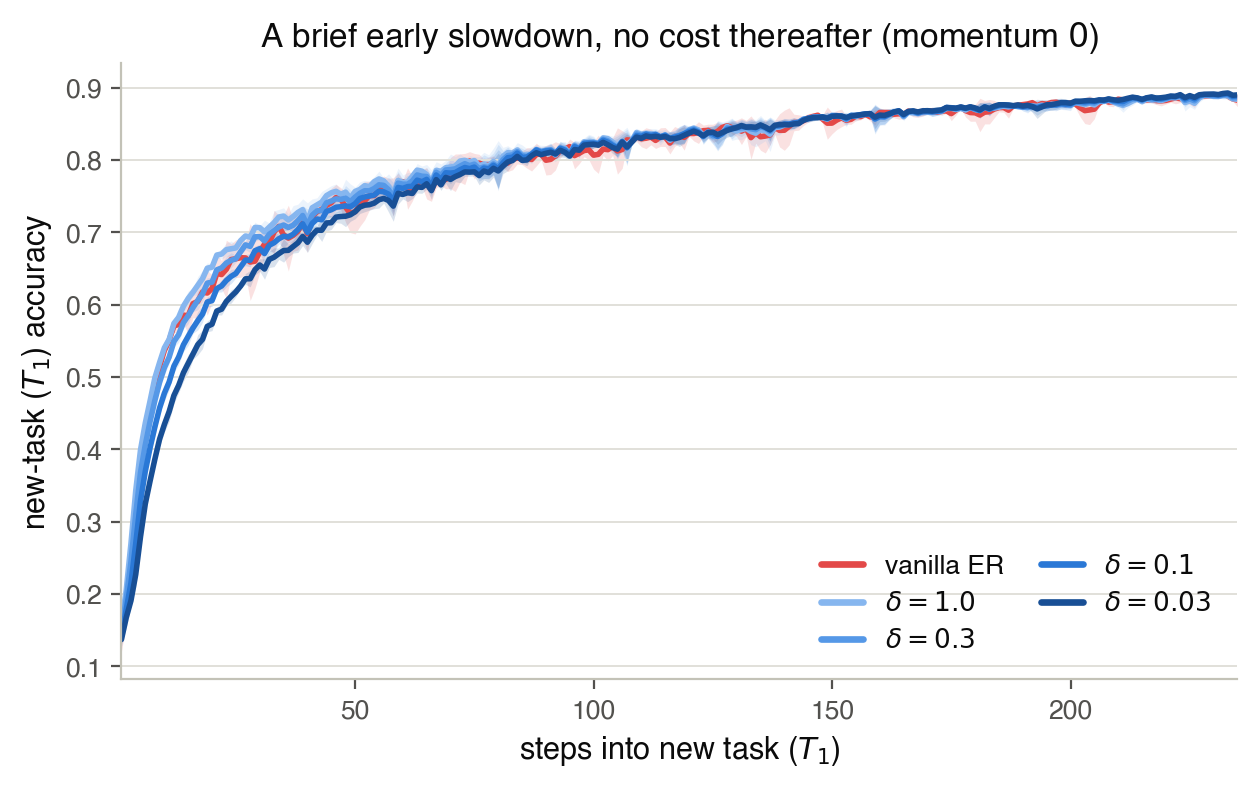
\includegraphics[width=0.8\linewidth]{img/results/asymmetric_per/per_plasticity.png}
    \caption{New-task ($T_1$) accuracy across the rot-MNIST switch at momentum $0$ for the standard-buffer $\delta$ sweep against vanilla ER (red); seed mean with $\pm$std bands. The strongest filter ($\delta{=}0.03$, darkest) lags briefly over the first ${\approx}50$ steps, the selective slowdown along past-task-sharp directions, and matches vanilla from then on; the plasticity metrics at horizon $100$ and beyond record no cost (Table~\ref{tab:res_per}).}
    \label{fig:per_plasticity}
\end{figure*}

\paragraph{The cliffs: an unexpected late failure.}
The one place the sweep breaks monotonicity is the strongest full-buffer setting, $\delta = 0.03$, where mean depth jumps to $9.5$ pp with a std of $8.2$: in $3$ of $5$ seeds the past-task curve holds flat for roughly two hundred steps and then slides off a late cliff, the red per-seed traces in Figure~\ref{fig:per_curves}(b). A solver control rules out the most straightforward explanation: rerunning the setting with the conjugate-gradient solver at $60$ iterations instead of $25$ reproduces the cliffs at the same seeds and steps ($11.5$ pp mean depth), so they are not an artefact of an under-converged solve. The cliffs came as a surprise: the account made no prediction of a late, abrupt failure, and nothing in the rest of the sweep hints at one. They are also confined to the exact-gradient diagnostic: at the same $\delta$ on the standard $1$k buffer no seed shows one (depth $4.8 \pm 1.9$ pp, the monotone end of the sweep). The failure is tied to the exact replay gradient: the sampling jitter of a practical buffer appears to protect against it, the same noise that elsewhere drives the overshoot here keeping the iterate from settling into the escape direction. Why the cliffs happen we can only partly say. A reading consistent with the data is a blind spot of the gate's model of the past task: the filter passes new-task pressure through directions its sampled Fisher rates as flat, and in these seeds that trust appears to be misplaced further out along the trajectory. We offer this as a hypothesis, not an established mechanism. What the control does establish is that the strongest filter can fail late and abruptly when nothing perturbs it. Because the failure is confined to the diagnostic leg, it is unlikely in a practical configuration, but it exposes a real weakness of feedforward control.

\paragraph{Momentum re-inflates the per-step filter.}
Momentum undoes the directional gate's protection, the opposite of what it does for the scalar gate, and it does so on both legs: on the practical $1$k buffer depth climbs from $4.8$ to $8.5$ pp at $\delta{=}0.03$ (Figure~\ref{fig:regime}), and on the full-buffer diagnostic from $2.2$ to $7.6$ pp at $\delta{=}0.1$ and from $1.5$ to $9.1$ pp at $\delta{=}0.3$ (both across all five seeds). Momentum accumulates the already-filtered direction, but the filter attenuates the step, not the source: the new-task loss, and with it the per-step gradient, keeps its full size, and because motion in the braked directions is slow, the shrunk push persists there step after step. A persistent push entering the accumulator is amplified toward $1/(1-\mu)$ times its per-step size, so velocity rebuilds displacement in the very directions the filter shrinks one step at a time. This re-inflation is what makes the head-to-head comparison of the next subsection regime-dependent.

\subsection{Reading the Momentum Crosses Together}
\label{subsec:res_regimeflip}

Read side by side in both gates' practical regime, the $1$k reservoir, the curriculum's and the directional gate's momentum crosses show that the two gates do not sit on a fixed stability--plasticity frontier a practitioner trades along: which gate leaves the smaller gap is decided by the momentum setting, the same setting that decides final accuracy. Figure~\ref{fig:regime} shows it directly, the same three methods at the same buffer with only the momentum setting changed between the panels.

\begin{figure*}[t]
    \centering
    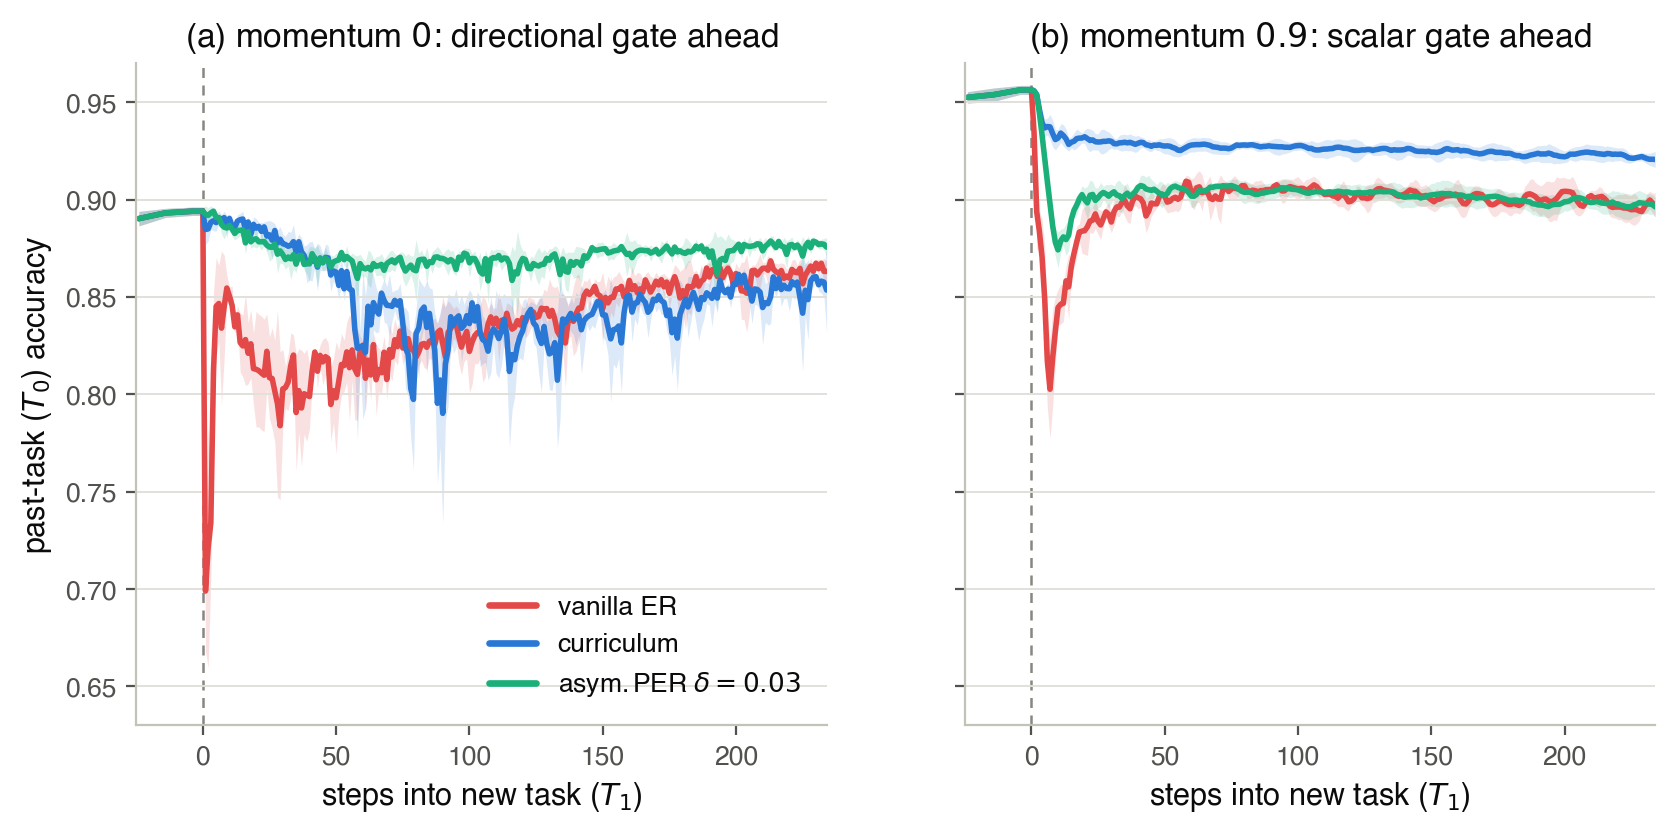
\includegraphics[width=0.85\linewidth]{img/results/momentum/regime_flip.png}
    \caption{The momentum synthesis at the matched $1$k buffer: per-step past-task ($T_0$) accuracy across the rot-MNIST switch for vanilla ER (red), the practical curriculum C7 (blue), and asymmetric PER at its strongest standard-buffer filter $\delta{=}0.03$ (aqua); seed mean with $\pm$std bands, $x{=}0$ the task switch. \textbf{(a) Momentum $0$:} the directional gate holds $T_0$ highest ($4.8$ pp / ACC $0.880$) while the curriculum opens a deep, noisy dip ($13.9$ pp / $0.837$). \textbf{(b) Momentum $0.9$:} the ordering swaps: the curriculum holds $T_0$ near its plateau ($3.7$ pp / $0.931$) while accumulated velocity re-inflates the directional gate's per-step filter ($8.5$ pp / $0.929$). The pre-switch level is higher in (b) because momentum converges $T_0$ higher before the switch.}
    \label{fig:regime}
\end{figure*}

At momentum $0$ the directional gate is better on both axes: $4.8$ pp of depth at $0.880$ accuracy against the curriculum's $13.9$ pp at $0.837$, with no measured plasticity debt to leave unpaid, and its one remaining cost is the per-step conjugate-gradient solve against the scalar gate's single gradient-norm ratio (Table~\ref{tab:res_cost}). Momentum, standard on realistic backbones and decisive for final accuracy at these budgets, reverses the ranking through the re-inflation mechanism above: the directional gate climbs to $8.5$ pp at the matched buffer while the curriculum, attenuating at source, reaches $3.7$ pp at vanilla accuracy, and with the buffers matched the directional gate has no accuracy advantage left to offset its re-inflated gap ($0.929$ vs.\ $0.931$). The choice between the gates is therefore not a point on a frontier but a consequence of whether momentum is on: off, take the directional gate; on, take the scalar gate. A five-task rot-MNIST sequence reproduces this picture across four consecutive boundaries: at momentum $0$ the directional gate keeps its edge, under momentum the curriculum keeps the least cumulative forgetting while the re-inflated directional gate falls back to vanilla ER's level (Appendix~\ref{app:longseq_full}, Figure~\ref{fig:longseq}).

\subsection{Generalisation to CIFAR-10 (RQ4)}
\label{subsec:res_cifar}

The CIFAR-10 block tests whether both gates carry to a ResNet-18, a clean $\rightarrow$ corruption shift, and the two normalisations that govern the post-switch recovery. Table~\ref{tab:res_cifar} reports the headline block at momentum $0.9$, the practically relevant regime.

\begin{table*}[htbp]
    \centering
    \small
    \begin{tabular}{ll cccc}
        \hline
        Norm & Method                                   & \texttt{gap\_depth} (pp) & \texttt{gap\_area\_end} & ACC               & min-ACC           \\
        \hline
        \multirow{3}{*}{BatchNorm}
             & G1: Vanilla ER                           & $11.8 \pm 2.5$           & $17.5 \pm 4.6$          & $0.723 \pm 0.008$ & $0.644 \pm 0.023$ \\
             & G2: Curriculum ($\lambda_{\min}{=}0.20$) & $\mathbf{4.8 \pm 0.7}$   & $\mathbf{3.6 \pm 2.2}$  & $0.722 \pm 0.011$ & $0.713 \pm 0.017$ \\
             & G3: Asym.\ PER ($\delta{=}0.1$)          & $5.9 \pm 4.3$            & $3.3 \pm 3.0$           & $0.715 \pm 0.011$ & $0.698 \pm 0.023$ \\
        \hline
        \multirow{3}{*}{GroupNorm}
             & G4: Vanilla ER                           & $41.2 \pm 13.5$          & $34.9 \pm 23.7$         & $0.730 \pm 0.011$ & $0.309 \pm 0.111$ \\
             & G5: Curriculum ($\lambda_{\min}{=}0.20$) & $\mathbf{5.2 \pm 2.1}$   & $\mathbf{1.7 \pm 0.9}$  & $0.731 \pm 0.020$ & $0.670 \pm 0.055$ \\
             & G6: Asym.\ PER ($\delta{=}0.1$)          & $5.6 \pm 1.1$            & $4.8 \pm 3.8$           & $0.741 \pm 0.009$ & $0.673 \pm 0.023$ \\
        \hline
    \end{tabular}
    \caption{CIFAR-10 headline block (ResNet-18, momentum $0.9$, buffer $5{,}000$, five seeds). Both gates cut gap depth and area far below vanilla ER at matched final accuracy and much higher worst-case retention (min-ACC), under both normalisations. Neither was given a CIFAR-specific sweep; both carry their rot-MNIST configurations.}
    \label{tab:res_cifar}
\end{table*}

\paragraph{Both gates carry to the deeper backbone.}
The rot-MNIST result carries over and strengthens. Under batch norm the curriculum cuts depth from $11.8$ to $4.8$ pp and asymmetric PER to $5.9$ pp; under group norm, where vanilla ER suffers a catastrophic $41.2$ pp drop, the curriculum cuts it to $5.2$ pp and asymmetric PER to $5.6$ pp. Every gate-vs-vanilla depth and area contrast holds across all five seeds, at final accuracy within about $0.01$ of vanilla and with worst-case retention sharply improved, min-ACC rising from $0.31$ to $0.67$ under group norm. On this backbone the transient stays open for hundreds of steps, so the area carries as much of the comparison as the depth (Figure~\ref{fig:cifar_curves}): vanilla ER under group norm crashes $T_0$ almost to chance and crawls back over the whole recovery window, while both gates hold $T_0$ near its plateau through the switch. At the matched $5{,}000$ buffer and momentum $0.9$ both gates land in the same few-pp band, with the curriculum the cheaper of the two (below), consistent with the momentum regime of Section~\ref{subsec:res_regimeflip}. The few-pp dip both gates keep under batch norm is boundary-localised and recovers within tens of steps, consistent with the running statistics re-adapting to the shifted inputs, a pathway no gate on the update touches (Appendix~\ref{app:cifar_headline_full}).

\begin{figure*}[t]
    \centering
    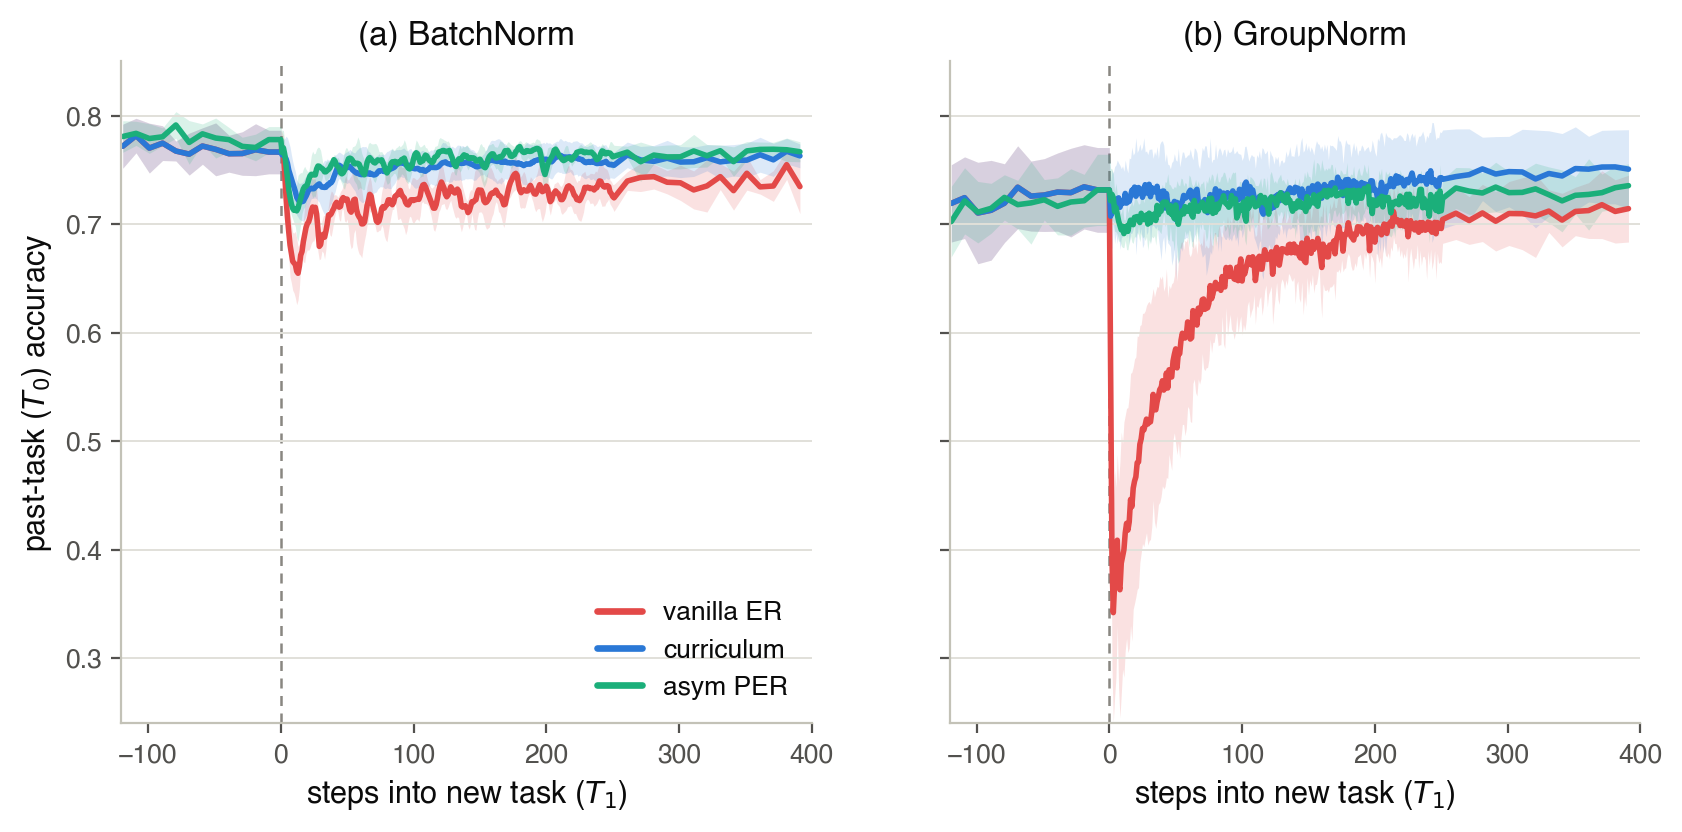
\includegraphics[width=0.85\linewidth]{img/results/cifar/cifar_headline.png}
    \caption{Per-step past-task ($T_0$) accuracy across the CIFAR-10 transition (ResNet-18, momentum $0.9$, buffer $5{,}000$), one panel per normalisation, each overlaying vanilla ER (red), the practical curriculum (blue) and asymmetric PER (aqua); seed mean with $\pm$std bands, $x{=}0$ the task switch. \textbf{(a) BatchNorm:} vanilla ER dips and re-adapts slowly while both gates hold $T_0$ near its plateau. \textbf{(b) GroupNorm:} vanilla ER's transient is deep and long, whereas both gates hold $T_0$ flat through the switch (Table~\ref{tab:res_cifar}, Appendix~\ref{app:cifar_headline_full}).}
    \label{fig:cifar_curves}
\end{figure*}

\paragraph{Mechanism, generalisation, and cost.}
Three further checks are reported in full in Appendix~\ref{app:cifar_extra}. A momentum cross on the deep backbone (Table~\ref{tab:res_cifar_mom}) turns out to be only weakly informative: at momentum $0$ the ResNet under-converges in ten epochs (vanilla ACC $0.65$, against $0.730$ with momentum), and on that degraded baseline both gates improve with momentum by similar margins ($28.6 \rightarrow 5.2$ pp for the curriculum, $22.6 \rightarrow 5.6$ pp for the directional gate), so the cross cannot separate the predicted composition from a general convergence gain; the vanilla depth null ($40.5 \rightarrow 41.2$ pp) sits on the same degraded baseline. The momentum signatures therefore rest on the rot-MNIST results, where the MLP isolates them cleanly (Section~\ref{subsec:disc_limits}). A generalisation block (Appendix~\ref{app:cifar_gen_full}, Table~\ref{tab:app_cifar_gen}) shows the curriculum beating a paired vanilla control on two corruptions it was never tuned on (shot noise $46.3 \rightarrow 7.3$ pp, contrast $8.4 \rightarrow 3.9$ pp under group norm), with a single three-task group-norm sequence flagged as a reliability boundary of the adaptive ratio when two consecutive corruptions are near-identical and both gradient norms become small (Figure~\ref{fig:failure_curves}; traced in Appendix~\ref{app:cifar_gen_full}). Finally, compute separates the gates where retention does not (Table~\ref{tab:res_cost}): the scalar gate is one gradient-norm ratio on top of a standard ER step and leaves the GPU half-idle, while the directional gate's $25$ conjugate-gradient Fisher-vector products per step saturate it, costing ${\sim}16\times$ the wall-clock and ${\sim}24\times$ the GPU energy on the ResNet-18 at similar peak memory; on the MLP both runs finish in under half a minute and the difference is negligible. In the momentum regime standard in practice, then, the scalar gate matches the directional gate's retention at essentially vanilla-ER cost and without the blind-spot cliffs, which is why it is the default recommendation.

\subsection{Summary of Findings}
\label{subsec:res_summary}

The account holds end to end, with one revision it forced. The gap separates into overshoot of the followed path and a deterministic arc of the intended one (RQ1), and the step-size ladder separates them as a limit: at momentum $0$ the excursion falls as $\eta \rightarrow 0$ but not to zero, converging on $3.8$ pp of depth and $0.34$ of flow-time area at ACC $0.898$ on the exact replay gradient ($4.7$ pp / $0.27$ / $0.877$ on the sampled buffer), so between two thirds and three quarters of the depth measured at the standard operating point is discretisation overshoot and the remainder is the path itself. That remainder is the revision the measurement forced on the account's metric mapping: depth is overshoot-dominated at the operating point but it is not overshoot alone. The arc is what the gates have to remove, and at the standard step size, where the ladder's own remedy costs a hundredfold longer run. The scalar feedback gate with momentum reaches $3.7$ pp of depth at vanilla accuracy, and C8 shows the pairing to be forced rather than fortunate, since the residual the schedule leaves at momentum $0$ is estimator variance and momentum is the variance reducer a $1$k memory can afford (RQ2); the directional feedforward gate shrinks depth and arc monotonically at no measured plasticity cost, but fails late and abruptly at its strongest diagnostic setting and re-inflates under momentum (RQ3); the comparison is therefore regime-dependent, and both gates carry to CIFAR-10 at matched accuracy and much improved worst-case retention (RQ4). The discussion reads these findings against the account of Section~\ref{sec:motivation}.
